	\documentclass[12pt]{book}
\usepackage[a4paper, total={6in, 8in}]{geometry}
\usepackage{amssymb}
\usepackage{listings}
\usepackage{color}
\usepackage{graphicx}
\usepackage{subfig}
\usepackage{float}
\definecolor{mygrey}{gray}{.96} % Light Grey
\definecolor{BrickRed}{RGB}{120,0,0}


\def\xbf{\mathbf{x}}
\def\zbf{\mathbf{z}}
\def\xibf{\mathbf{\xi}}
\lstset{
	language=R,              % choose the language of the code ("language=Verilog" is popular as well)
   tabsize=3,							  % sets the size of the tabs in spaces (1 Tab is replaced with 3 spaces)
	basicstyle=\footnotesize,               % the size of the fonts that are used for the code
	numbers=left,                   % where to put the line-numbers
	numberstyle=\footnotesize,              % the size of the fonts that are used for the line-numbers
	stepnumber=1,                   % the step between two line-numbers. If it's 1 each line will be numbered
	numbersep=5pt,                  % how far the line-numbers are from the code
	backgroundcolor=\color{mygrey}, % choose the background color. You must add \usepackage{color}
	showspaces=false,              % show spaces adding particular underscores
	showstringspaces=false,        % underline spaces within strings
	showtabs=false,                % show tabs within strings adding particular underscores
	frame=single,	                 % adds a frame around the code
	tabsize=3,	                    % sets default tabsize to 2 spaces
	captionpos=b,                   % sets the caption-position to bottom
	breaklines=true,                % sets automatic line breaking
	breakatwhitespace=false,        % sets if automatic breaks should only happen at whitespace
	%escapeinside={\%*}{*)},        % if you want to add a comment within your code
	commentstyle=\color{BrickRed}   % sets the comment style
}

\begin{document}
\title{\textbf{Monte Carlo Simulation Lab Assignment-9}}
\author{Yash Vanjani\\(140123046)\\Mathematics and Computing\\IIT Guwahati}
\date{April 12th, 2016}

\maketitle

\newpage
\begin{enumerate}
\item[Q 1] Generate 10 sample paths for the standard Brownian Motion in the time interval [0, 5]
using the recursion
$$W (t_{i+1} ) = W (t_i ) + \sqrt{t_{i+1} - t_i} * Z_{i+1}$$
with 5000 generated values for each of the paths where $Z_{i+1} \sim N (0, 1)$. Plot all the
sample paths in a single figure. Also estimate E[W(2)] and E[W(5)] from the 10 paths
that you have generated.
\end{enumerate}
\noindent{Code for R}

\begin{lstlisting}
library(stats)
w<-vector("numeric")
t<-vector("numeric")
pal<- palette()
t[1]=0
sec2<-vector("numeric") #for storing BM values at 2nd sec
sec5<-vector("numeric") #for storing BM values at 5th sec
for(i in 1:4999)
{
	t[i+1]=t[i]+0.001
}
for(i in 1:10)
{
	z<-rnorm(5000, mean=0, sd=1)
	w[1]=0
	for (j in 1:4999)
	{
		w[j+1]=w[j]+z[j+1]*sqrt(0.001)
		if(j==2000)
		{
			sec2[i]=w[2000]
		}
		if(j==4999)
		{
			sec5[i]=w[5000]
		}

	}
	if(i==1)
	{
		plot(t,w,type="l", col=pal[i %% 8 +1],ylim=c(-5,5))
	}
	else
	{
		lines(t,w, col=pal[i %% 8 +1],ylim=c(-5,5))
	}
}
cat("E[W(2)] = ",mean(sec2),"\n")
cat("E[W(5)] = ",mean(sec5),"\n")
\end{lstlisting}
\textbf{\underline{Output:}} \\\\
$E[W(2)] =  -0.0492709$ \\
$E[W(5)] =  -0.02063341$ \\\\
The corresponding plot of "W v/s t" is shown below:
\begin{figure}[H]
	\centering
	\subfloat["W v/s t" plot]{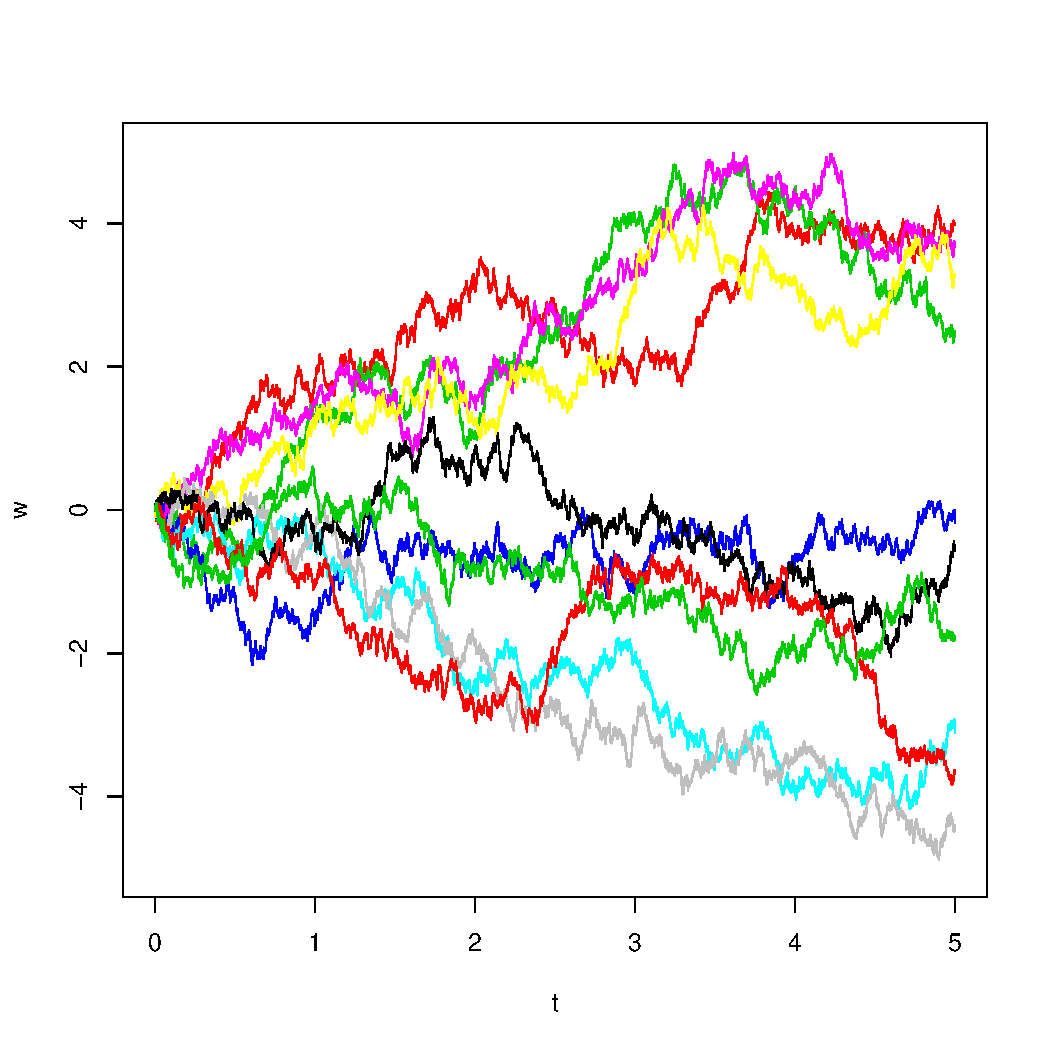
\includegraphics[width=0.9\textwidth]{1.pdf}}	
\end{figure}

\newpage
\begin{enumerate}
\item[Q 2] Repeat the above exercise with the following Brownian motion (BM(μ, σ 2 )) discretization $X(t_{i+1}) = X(t_i ) + \mu(t_{i+1} - t_i ) + \sigma \sqrt{ t_{i+1} - t_i}* Z_{i+1}$ . Take $X(0) = 5$, $\mu = 0.06$ and $\sigma = 0.3$
\end{enumerate}
\noindent{Code for R}

\begin{lstlisting}
library(stats)
x<-vector("numeric")
t<-vector("numeric")
pal<- palette()
t[1]=0
sec2<-vector("numeric") #for storing BM values at 2nd sec
sec5<-vector("numeric") #for storing BM values at 5th sec
for(i in 1:4999)
{
	t[i+1]=t[i]+0.001
}

mu<-0.06
sigma<-0.3

for(i in 1:10)
{
	z<-rnorm(5000, mean=0, sd=1)
	x[1]=5
	for (j in 1:4999)
	{
		x[j+1]=x[j]+(z[j+1]*sqrt(0.001)*sigma)+(mu*0.001)
		
		if(j==2000)
		{
			sec2[i]=x[2000]
		}
		if(j==4999)
		{
			sec5[i]=x[5000]
		}

	}
	if(i==1)
	{
		plot(t,x,type="l", col=pal[i %% 8 +1],ylim=c(2,8))
	}
	else
	{
		lines(t,x, col=pal[i %% 8 +1],ylim=c(2,8))
	}
}
cat("E[W(2)] = ",mean(sec2),"\n")
cat("E[W(5)] = ",mean(sec5),"\n")
\end{lstlisting}
\textbf{\underline{Output:}} \\\\
E[W(2)] =  5.075252 \\
E[W(5)] =  5.301343 \\\\
The corresponding plot of "X v/s t" is shown below:
\begin{figure}[H]
	\centering
	\subfloat["X v/s t" plot]{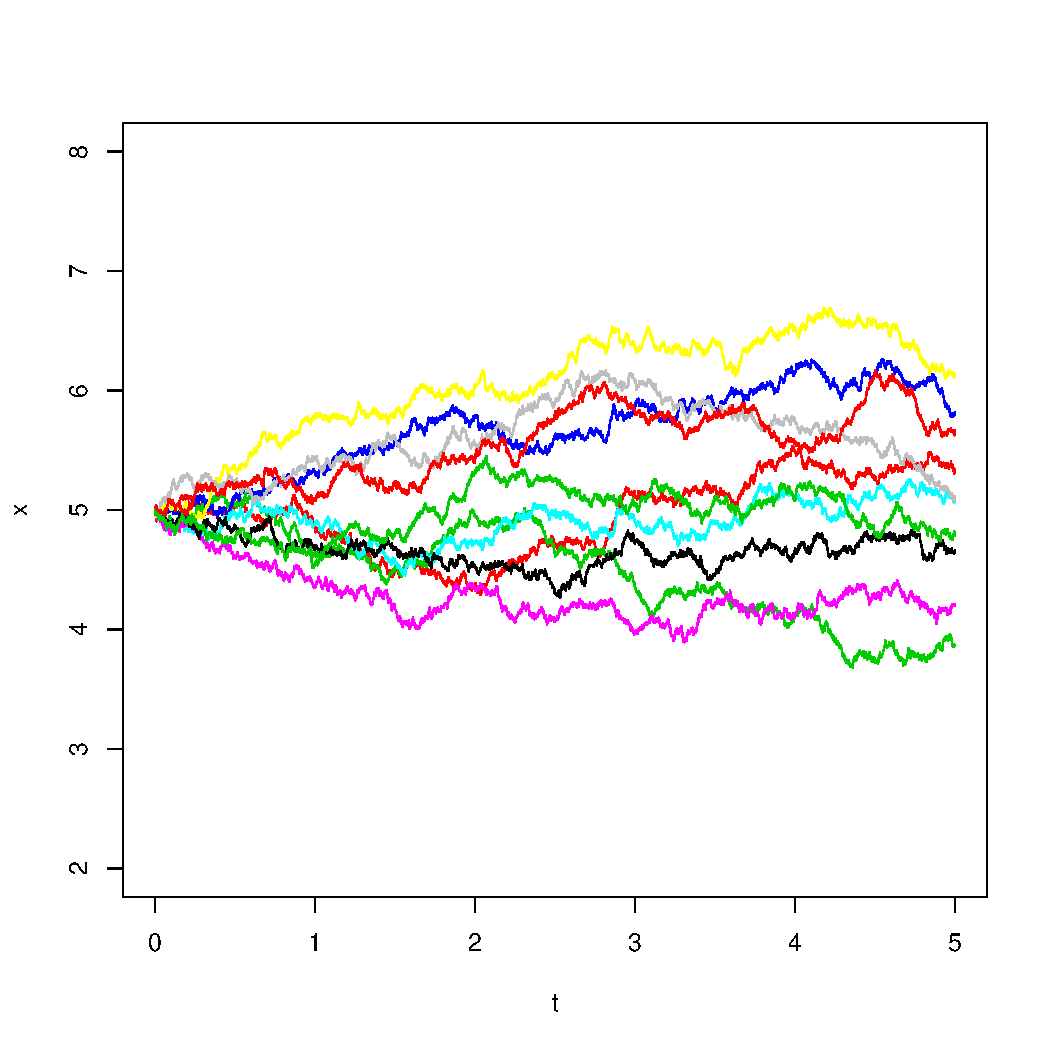
\includegraphics[width=0.9\textwidth]{2.pdf}}	
\end{figure}
\newpage
\begin{enumerate}
\item[Q 3] The Euler approximated recursion with time dependent $\mu$ and $\sigma$ is given by:
$$Y (t_{i+1} ) = Y (t_i ) + \mu(t_i )(t_{i+1} - t_i ) + \sigma(t_i) \sqrt{t_{i+1} - t_i}*Z_{i+1}$$
Repeat the above exercise by taking
$$Y (0) = 5, \mu(t) = 0.0325 - 0.05t, \sigma(t) = 0.012 + 0.0138t + 0.00125t^2 .$$
\end{enumerate}
\noindent{Code for R}

\begin{lstlisting}
library(stats)
Y<-vector("numeric")
t<-vector("numeric")
pal<- palette()
t[1]=0
sec2<-vector("numeric") #for storing BM values at 2nd sec
sec5<-vector("numeric") #for storing BM values at 5th sec
mu<-vector("numeric")
sigma<-vector("numeric")
for(i in 1:4999)
{
	t[i+1]=t[i]+0.001
}
for(i in 1:5000)
{
	mu[i]=0.0325-(0.05*(t[i]))
	sigma[i]=0.012+(0.0138*t[i])+(0.00125*t[i]*t[i])
}

for(i in 1:10)
{
	z<-rnorm(5000, mean=0, sd=1)
	Y[1]=5
	for (j in 1:4999)
	{
		Y[j+1]=Y[j]+(z[j+1]*sqrt(0.001)*sigma[j])+(mu[j]*0.001)
		
		if(j==2000)
		{
			sec2[i]=Y[2000]
		}
		if(j==4999)
		{
			sec5[i]=Y[5000]
		}

	}
	if(i==1)
	{
		plot(t,Y,type="l", col=pal[i %% 8 +1],ylim=c(4,6))
	}
	else
	{
		lines(t,Y, col=pal[i %% 8 +1],ylim=c(4,6))
	}
}
cat("E[W(2)] = ",mean(sec2),"\n")
cat("E[W(5)] = ",mean(sec5),"\n")
\end{lstlisting}
\textbf{\underline{Output:}} \\\\
E[W(2)] =  5.075252 \\
E[W(5)] =  5.301343 \\\\
The corresponding plot of "Y v/s t" is shown below:
\begin{figure}[H]
	\centering
	\subfloat["Y v/s t" plot]{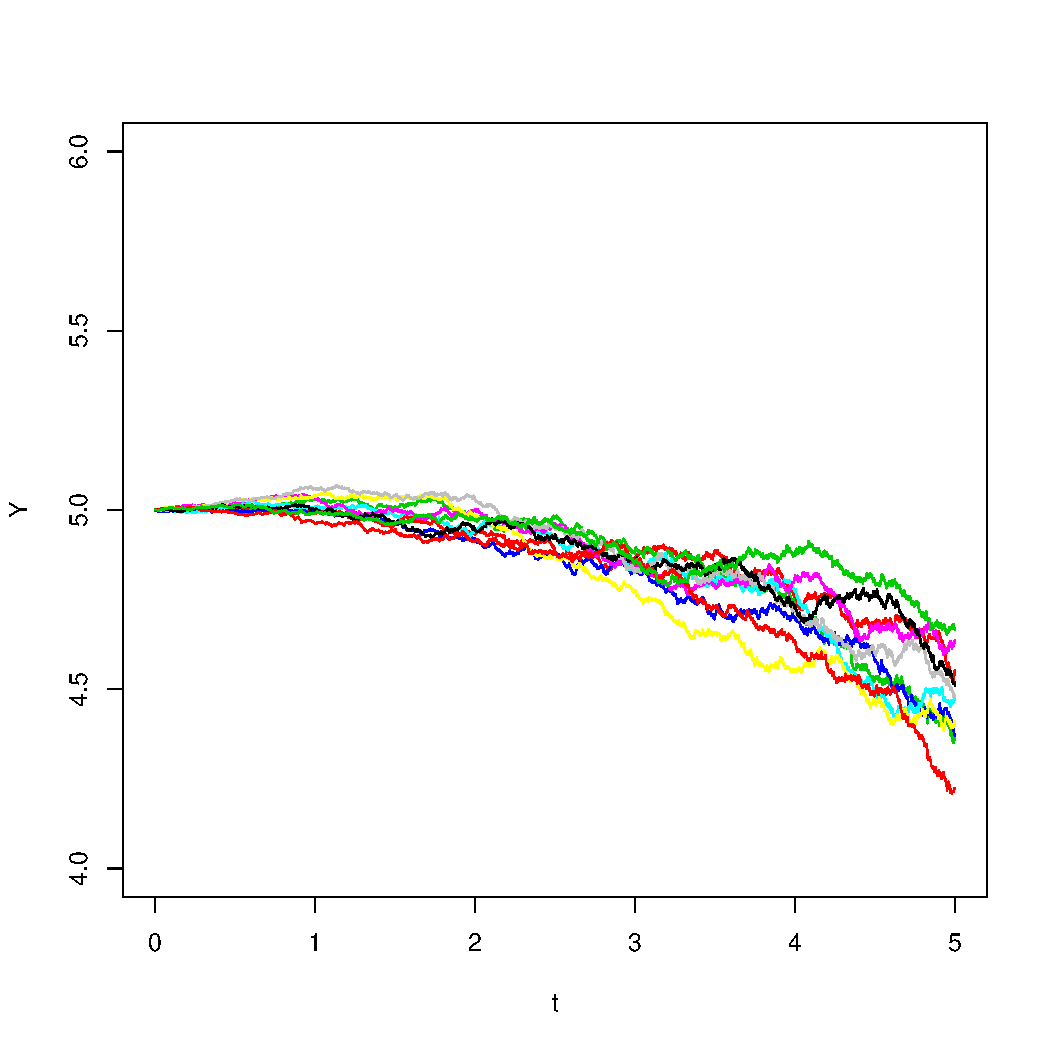
\includegraphics[width=0.75\textwidth]{3.pdf}}	
\end{figure}
\end{document}
